% !TeX root = ../apuntes-ea.tex

\chapter{Clasificación de grupos de orden pequeño}

El objetivo final de la teoría de grupos es clasificar los grupos según sus propiedades. Durante el resto del curso veremos formas cada vez más sofisticadas de clasificar los grupos. Empezaremos con algunos resultados que permiten clasificar grupos finitos de orden pequeño.

\section{Producto directo de grupos}

El producto directo de grupos permite generar otro grupo a partir de otros.

\begin{dfn}[Producto directo de grupos]
	Sean $(G_1, \ast), (G_2, \bullet)$ grupos. Llamamos producto directo de los grupos $G_1$ y $G_2$ al grupo $(G_1\times G_2, \sim)$. Donde $\sim : (G_1 \times G_2) \times (G_1 \times G_2) \to G_1 \times G_2,\ (g_1, g_2) \sim (g_1', g_2') = (g_1\ast g_1', g_2 \bullet g_2')$.
	
	En general, dados $(G_1, \ast_1),\dots, (G_n, \ast_n)$ podemos definir el producto directo con
	\begin{align*}
		(G_1, \ast_1) \times \dots (G_n, \ast_n) = \varprod_{i=1}^n (G_i, \ast_i) = \left(\varprod_{i=1}^n G_i, \sim\right)
	\end{align*}
	donde $\sim: (\varprod_{i=1}^n G_i) \times (\varprod_{i=1}^n G_i) \to \varprod_{i=1}^n G_i$ con $(g_1, \dots, g_n) \sim (g'_1, \dots, g'_n) = (g_1 \ast_1 g'_1, \dots, g_n \ast_n g'_n)$.
\end{dfn}

Cuando se utiliza la notación aditiva es común llamarlo suma directa.

\begin{dfn}[Suma directa]
	Sean $(G_1, +), \dots, (G_n, +)$ grupos cuya operación es la suma\footnote{Lo importante es que es la misma operación para todos y que utilizamos la notación aditiva, lo que \textit{suma} signifique en realidad nos importa poco} entonces denotamos por suma directa al producto directo de todos ellos:
	\begin{align*}
		\bigoplus_{i=1}^n (G_i, +) = \left(\bigoplus_{i=1}^n G_i, \oplus\right) = (G_1 \times \dots \times G_n, \oplus)
	\end{align*}
	donde $\oplus: (\bigoplus_{i=1}^n G_i) \times (\bigoplus_{i=1}^n G_i) \to \bigoplus_{i=1}^n G_i$ se define con $g \oplus g' = (g_1 + g'_1, \dots, g_n + g'_n)$.
\end{dfn}

El producto directo se trata con detalle más adelante pero aquí van un par de teoremas.

\begin{thm}
	Sean $n, m \in \N$. El grupo producto directo $\ZnZ \times \ZmZ$ es cíclico $\iff mcd(n,m) = 1$.
\end{thm}

\begin{proof}
	Para que $\ZnZ \times \ZmZ$ sea cíclico debe haber un elemento $a \in \ZnZ \times \ZmZ \mid o(a) = m\cdot n$. Si $m$ y $n$ no son coprimos entonces el orden de $a$ no puede ser $m\cdot n$. %TODO pensar y explicar
\end{proof}

Este teorema puede ser útil combinado con el resultado anterior (\autoref{thm:clasificacionciclicos}), para dar isomorfismos a productos directos que sean cíclicos.

\begin{thm}
	\label{thm:noprobado1}
	Si $G$ es abeliano y $|G| < \infty$ entonces $G$ es un producto de grupos cíclicos finitos.
\end{thm}

\begin{proof}
	Dice que no lo vamos a probar, pero veremos algunos resultados más adelante (en la sección sobre clasificación de grupos finitos \ref{gruposfinitosnotables}).
\end{proof}


\section{Producto libre de grupos}

\begin{dfn}[Producto libre de grupos]
	\label{dfn:productolibre}
	Sean $S,T$ subconjuntos del grupo $G$. Definimos $ST = \{s\ast t \mid s \in S \land t \in T\}$.
\end{dfn}

Es importante remarcar el \textbf{el producto libre de [sub]grupos no siempre es un grupo, a diferencia del producto libre que siempre funciona. En general solo es un conjunto.} Ver el teorema \ref{thm:condicionproductolibre}

Observemos que la función $f: S \times T \to ST,\ (s,t) \mapsto st$ no es un homomorfismo de grupos. Esto es porque al operar dos elementos de $S \times T$ no se comporta bien. Sean $s,s'\in S, t,t'\in T$
\begin{align*}
(s,t) \mapsto st \\
(s',t') \mapsto s't' \\
\end{align*}
esperamos que 
\begin{align*}
f((s,t)(s',t')) = f(st, s't') \mapsto f(s,t)f(s',t') = sts't'
\end{align*}
pero en realidad ocurre que
\begin{align*}
f((s,t),(s',t')) \mapsto ss'tt' \neq f(s,t)f(s',t')
\end{align*}

No obstante, aunque la función que lleva $H_1 \times H_2 \to H_1 H_2$ no sea un homomorfismo, sí podemos saber cuantos elementos tiene $H_1H_2$.

\begin{thm}[Cardinalidad del producto libre]
	\label{thm:cardinalidadproductolibre}
	Sean $H_1, H_2 < G$ con $G$ finito. Entonces
	\begin{align}
	|H_1H_2| = \frac{|H_1||H_2|}{|H_1 \cap H_2|}
	\end{align}
\end{thm}

\begin{proof}
	Utilizaremos la función $f:H_1 \times H_2 \to H_1 H_2$ que es sobreyectiva por definición de $H_1 H_2$. Para una función sobreyectiva $f: A \to B,\ |A| = \sum_{b \in B} |f^{-1}(b)|$.
	
	%TODO argumentar lo del alpha
	
	Sean las fibras los conjuntos $f^{-1}(h_1h_2)$ de los pares de elementos que van a parar al mismo $h_1h_2 \in H_1 H_2$. La condición necesaria y suficiente para que $(h_1', h_2')$ esté en la misma fibra que $(h_1, h_2)$ es que $h_1' = h_1 \alpha \land h_2' = h_2 \alpha,\ \alpha \in H_1 \cap H_2$. Entonces $|f^{-1}(h_1, h_2)| = | (h_1 \alpha, h_2\alpha),\ \alpha \in H_1\cap H_2| = |H_1 \cap H_2| \implies |H_1||H_2| = |H_1 H_2| |H_1 \cap H_2|$ 
\end{proof}

\begin{thm}
	\label{thm:condicionproductolibre}
	Sean $H_1, H_2$ subgrupos de $G$, con $G$ finito. Si $H_2 \normsub G$ entonces $H_1 H_2 < G$ (si uno de los subgrupos es normal, entonces el producto es subgrupo).
\end{thm}

\begin{proof}
	Observamos que podemos escribir $H_1H_2 = \bigcap_{h \in H_1} h \ast H_2$. Como $H_2 \normsub G,\ h\ast H_2 \cdot h' H_2 = h h' H_2\ \forall h \in H_1$. Si nos fijamos $H_1 H_2$ es cerrado por la operación pues $h h' H_2 \in H_1H_2$ y como $G$ es finito y por tanto $H_1, H_2$ también, $H_1H_2$ es un subgrupo.	
\end{proof}

\begin{thm}
	Si $H_1 \normsub G \land H_2 \normsub G \implies H_1 H_2 \normsub G$ (si los dos subgrupos son normales, enotnces el producto también es normal).
\end{thm}

\begin{proof}
	$H_1,H_2 < G$ luego $\forall g \in G,\ gH_1H_2g^{-1} = gH_1g^{-1}gHg^{-1}  = H_1 H_2 $.
\end{proof}


\section{Clasificación de grupos finitos}

\subsection{Teorema de clasificación de grupos finitos de orden pequeño}

\label{gruposfinitosnotables}

\begin{thm}[Grupos notables de distintos órdenes finitos.]$ $\newline
	\label{thm:clasificacionfinitos}
	
	\begin{itemize}
		\item $|G| = 2, 3, 5, 7, 11 \dots, p$ donde $p$ es primo:
		\begin{itemize}
			\item Abelianos cíclicos: son isomorfos con $\Z/p\Z$.
			\item Abelianos no cíclicos: no hay, por el corolario del teorema de Lagrange \ref{thm:lagrange}.
		\end{itemize}
		\item $|G| = 4$:
		\begin{itemize}
			\item Abelianos cíclicos: son isomorfos con $\Z/4\Z$
			\item Abelianos no cíclicos: son isomorfos con $\Z/2\Z \times \Z/2\Z$.
			\item No abelianos: no hay grupos no abelianos de orden menor que 4.
		\end{itemize}
		\item $|G| = 6$:
		\begin{itemize}
			\item Abelianos cíclicos: son isomorfos con $\Z/6\Z$.
			\item Abelianos no cíclicos: no hay porque todo grupo abeliano cuyo orden se puede descomponer en dos primos es cíclico (ver Hoja 1 ejercicio 19).
			\item No abelianos: todos son isomorfos con $D_3 \isom S_3$ (ver ejemplo \ref{ej:orden6noabisomd3}).
		\end{itemize}
		\item $|G| = 8$:
		\begin{itemize}
			\item Abelianos cíclicos: son isomorfos con $\Z/8\Z$.
			\item Abelianos no cíclicos: son isomorfos o bien con $\Z/4\Z \times \Z/2\Z$ o bien con $\Z/2\Z \times \Z/2\Z \times \Z/2\Z$ (depende de los órdenes de los elementos de $G$).
			\item No abelianos: son isomorfos o bien con el famoso grupo $D_4$ (ver ejemplo \ref{ej:famosogrupod4}) o bien con el grupo de cuaterniones $H$ (ver ejemplo \ref{ej:grupocuaterniones}). Ver ejemplo \ref{ej:orden8noabisom}
		\end{itemize}
	\end{itemize}
	
\end{thm}

\begin{proof}
	En lo que resta de sección se dan algunos ejemplos de los razonamientos que llevan a estas afirmaciones.
\end{proof}

Vamos a aplicar el teorema \ref{thm:noprobado1} a grupos abelianos.

\begin{thm}
	Sea $G$ abeliano con $|G| = p_1^{\alpha_1}p_2^{\alpha_2}\dots p_n^{\alpha_n}$. Entonces
	\begin{align}
	G \isom \Z/p_1^{\beta_{11}}\Z \times \Z/p_1^{\beta_{1s_1}}\Z \times \dots \Z/p_n^{\beta_{n1}}\Z \times \Z/p_1^{\beta_{ns_n}}\Z \text{ donde } \alpha_i = \sum_{j = 1\dots s_i} \beta_{ij}
	\end{align}
\end{thm}

En particular, se cumple que para grupos cíclicos $G$ de orden $n$, donde $G \isom \ZnZ$.

\begin{thm}
	\label{thm:znzisomproductodirecto}
	Sea un número y su factorización en primos: $n = p_1^{\alpha_1}p_2^{\alpha_2}\dots p_n^{\alpha_n}$. Entonces
	\begin{align}
	\ZnZ \isom \Z/p_1^{\alpha_1}\Z \times \Z/p_2^{\alpha_2}\Z \times \dots \times \Z/p_n^{\alpha_n}\Z
	\end{align}
\end{thm}

\begin{proof}
	Sea $d$ tal que $d \divides n$ y $n = dn'$. Por tanto $n' = p_2^{\alpha_2}\dots p_n^{\alpha}$ y $d = p_1^{\alpha_1}$. Como $\ZnZ = \{0, 1, 2, \dots, n', \dots, n-1\}$ tenemos que $o(n') = p_1^{\alpha_1}$. Luego $H = \langle n' \rangle$ es el único subgrupo de orden $p_1^{\alpha_1}$ y $N = \langle p_1^{\alpha_1} \rangle$ es el único subgrupo de orden $n'$. Ahora bien, por cómo hemos elegido $n'$ y $d$, $mcd(n', d) = 1$ por lo que $\ZnZ \isom \Z/d\Z \times \Z/n'\Z$. Podemos repetir este procedimiento hasta que descompongamos $n$ en potencias de primos y tendremos que $mcd(p_1^{\alpha_1}, p_2^{\alpha_2}, \dots, p_n^{\alpha_n}) = 1$ y por tanto $\ZnZ \isom \Z/p_1^{\alpha_1}\Z \times \Z/p_2^{\alpha_2}\Z \times \dots \times \Z/p_n^{\alpha_n}\Z$
\end{proof}

Lo que nos dice este teorema es que si un grupo es cíclico de orden $n$ entonces es isomorfo a $\ZnZ$ y a su vez a un producto directo en el que cada uno de los factores tiene como orden un factor de $n$, sin separarlos con la multiplicidad.

\begin{ej}
	Si un grupo de orden $12$ es cíclico entonces es isomorfo a $\Z/4\Z \times \Z/3\Z$, y no es isomorfo a $\Z/2\Z \times \Z/2\Z \times \Z/3\Z$.
\end{ej}

\begin{thm}
	Sea $G$ abeliano donde $|G| = r\cdot s$ con $mcd(r,s) = 1$ y ean $K < G \land N < G$ donde $|K| = r \land |N| = s$. Entonces $G \isom K \times N$.
\end{thm}

\begin{proof}
	Sabemos que $f:K\times N \to G,\ (k, h) \mapsto kh$ es un homomorfismo y por tanto $\ima f < G$. Para probar que $f$ es un isomorfismo probaremos que $\ima f = G$. Como $|K| = r \land |N| = s$ y $r$ y $s$ son coprimos entonces $K \cap N = \{e\}$. Por tanto $|K \cap N| = 1$ y utilizando el teorema \ref{thm:cardinalidadproductolibre} tenemos que $|KN| = \frac{|K||N|}{|K \cap N|} = |K| |N| = rs$ por lo que $f$ es sobreyectiva, y, por tanto, biyectiva, es decir, que $f$ es un isomorfismo.
\end{proof}

\begin{ej}
	Podemos afirmar que si $|G| = 6$ y $G$ es abeliano entonces $G \isom \Z/6\Z \isom \Z/2\Z \times \Z/3\Z$.
\end{ej}

Observemos que la hipótesis de abeliano es fundamental (ver ejemplo \ref{ej:nohomoentreproducto}).



\begin{ej}
	\label{ej:orden6noabisomd3}
	Sea $G$ no abeliano con $|G| = 6$. Entonces $G \isom D_3$.
\end{ej}

\begin{proof}
	\begin{enumerate}
		\item $G$ no abeliano $\implies G$ no cíclico $\implies \exists g \in G \mid o(g) \neq 6$
		\item $G$ no abeliano $\implies \exists b \in G \mid o(b) \neq 2 \implies o(b) = 3$ ya que si $b \in G$ entonces $o(b) \divides |G|$ (corolario teorema de Lagrange (\ref{thm:lagrange})).
		\item Sabemos pues que $\langle b \rangle = \{1, b, b^2\} < G$ y $|\langle b \rangle| = 3 \implies [G:\langle b \rangle] = \frac{|G|}{|\langle b \rangle|} = 2$. Es decir, que hay otra caja disjunta en la partición a la que llamamos $K$
		\item Por el teorema del cardinal del producto libre (teorema \ref{thm:cardinalidadproductolibre}) tenemos que $6 \geq |HK| = \frac{|H||K|}{|\langle b \rangle \cap K}$. Como $\langle b \rangle \cap K = \{e\}$ por ser las cajas disjuntas tenemos que $|K| = 2$ ya que si fuera $|K| = 3$ tendríamos que $|HK| = 9 \not \leq 6$.
		\item Definimos $\phi_a(x) : G \to G,\ x \mapsto ax\inv{a}$ (el isomorfismo de conjugación). $\phi_a$ es un isomorfismo, incluso cuando lo restringimos a un subgrupo normal. El subgrupo $\langle b \rangle$ es normal porque tiene índice 2 (ver teorema \ref{thm:indice2normal}).
		\item Por ello tenemos que si $\phi_a(x) = y$ entonces tiene que ser $o(x) = y$. Por tanto, aplicando $\phi_a$ a $b$ tenemos lo siguiente:
		\begin{align*}
		\phi_a(b) = ab\inv{a} = b \implies ab = ba \implies G \text{ abeliano} \\
		\phi_a(b) = ab\inv{a} = \inv{b} \implies ab = b^2a \implies ba = ab^2
		\end{align*}
		\item La primera no puede ser por hipótesis. La segunda nos da el final de la presentación de $D_3$:
		\begin{align*}
		D_3 = \langle a, b \rangle \text{ donde } o(a) = 2,\ o(b) = 3,\ ba = ab^2
		\end{align*}
	\end{enumerate}
\end{proof}

\begin{ej}
	\label{ej:orden8noabisom}
	Probar que si $G$ es un grupo no abeliano con $|G| = 8$ entonces o bien $G \isom D_4$ o bien $G \isom H$ donde $H$ es el grupo de cuaterniones (ver ejemplo \ref{ej:grupocuaterniones}).
\end{ej}

\begin{proof}$ $\newline
	\begin{enumerate}
		\item Tenemos que $G$ no es abeliano. Por el contrarrecíproco del teorema \ref{thm:ciclicoimplicaabeliano} tenemos que no puede ser cíclico por lo que $\not\exists g \in G \mid o(g) = 8$.
		\item Por el teorema \ref{thm:abelianosdeorden2} sabemos que $\exists b \in G \mid o(b) \neq 2 \implies \mathbf{o(b) = 4}$.
		\item Por el teorema de Lagrange \ref{thm:lagrange} sabemos que dicho $b$ tiene que tener $o(b) = 4$ ya que $\forall b \in G, o(b) \divides |G|$. Por tanto $\langle b \rangle = \{1, b, b^2, b^3\}$.
		\item Como $\langle b \rangle$ tiene orden $4$, el índice es $[G: \langle b \rangle] = 2$ por lo que hay otro subgrupo en $G$ disjunto a $\langle b \rangle$. Sea $a$ un elemento de dicho subgrupo.
		\item Fijado $a$, definimos el isomorfismo de conjugación $\phi_a: G \to G,\ \phi_a(x) = ax\inv{a}$. Este isomorfismo sigue siendo un isomorfismo cuando lo restringimos a un subgrupo normal como es el caso de $\langle b \rangle$ (ver teorema \ref{thm:indice2normal}).
		\item Para $b \in G$ pueden ocurrir las siguientes, porque $\phi_a$ debe mantener los órdenes por ser isomorfismo:
		\begin{itemize}
			\item $\phi_a(b) = ab\inv{a} = b \implies ab = ba \implies G$ abeliano. Descartamos esta opción por hipótesis.
			\item $\phi_a(b) = ab\inv{a} = \inv{b} \implies \mathbf{ba = a\inv{b} = ab^3}$
		\end{itemize}
		\item Ahora consideramos los posibles órdenes de $a$ que pueden ser $2$ o $4$ por el teorema de Lagrange:
		\begin{itemize}
			\item Si $\mathbf{o(a) = 2}$ entonces $G \isom D_4\ \qed$
			\item Si $\mathbf{o(a) = 4}$ entonces $\langle a \rangle = \{1, a, a^2, a^3\}$.
			\begin{enumerate}
				\item Miramos $\langle a \rangle \cap \langle b \rangle = \{1, a, a^2, a^3\} \cap \{1, b, b^2, b^3\} = \{1\} \implies |\langle a \rangle \cap \langle b \rangle| = 1$
				\item Por el teorema del orden del producto libre \ref{thm:cardinalidadproductolibre} tenemos que $|\langle a \rangle \langle b \rangle| = |\langle a \rangle ||\langle b \rangle| = 4 \cdot 4 = 16$, pero esto no puede ocurrir puesto que el orden del producto puede ser como máximo $8$. Es decir, que $\langle a \rangle \cap \langle b \rangle \neq \{e\}$.
				\item Ahora bien, la intersección de subgrupos debe ser un subgrupo, luego el orden debe ser divisor del orden de los grupos intersecados. El orden de $\langle a \rangle \cap \langle b \rangle$ puede ser 1, 2 o 4.
				\item Ya hemos visto que no puede ser 1. Tampoco puede ser 4 porque... por qué? Luego $o(\langle a \rangle \cap \langle b \rangle) = 2$ por lo que $\langle a \rangle \cap \langle b \rangle$ tiene 2 elementos.
				\item Uno de ellos es el neutro ($1$). El otro no puede ser ni $a$, ni $b$ porque al tener estos orden 4 tendría que haber más elementos. Tampoco puede ser ni $a^3$, ni $b^3$ porque también tienen orden 4 por el teorema \ref{thm:coprimosgeneradosiguales}. Luego $\langle a \rangle \cap \langle b \rangle = \{1, a^2\} = \{1, b^2\} \implies \mathbf{a^2 = b^2}$.
				\item Recopilando $o(a) = 4,\ o(b) = 4,\ a^2 = b^2,\ ba = a\inv{b}$ tenemos que $G \isom H \qedhere$
			\end{enumerate}
		\end{itemize}
	\end{enumerate}
\end{proof}

\section{Extra}

\begin{ej}[Retículo de subgrupos de $D_4$]
	Dar el retículo de subgrupos de $D_4 = \{1, B, B^2, B^3, A, AB, AB^2, AB^3\}$, donde $o(A) = 2,\ o(B) = 4,\ BA=AB^3$. En este caso no tenemos más remedio que ir probando a ver qué combinaciones de elementos dan subgrupos. Como conocemos de dónde viene $D_4$ nos es más fácil (ver el ejemplo \ref{ej:famosogrupod4}).
	
	\begin{figure}[h]
		\centering
		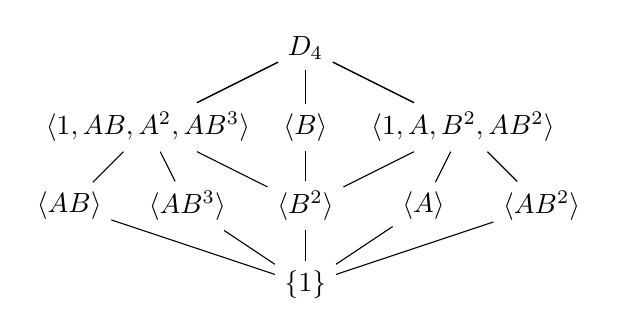
\begin{tikzpicture}
		\node (d4) at (0, 3) {$D_4$};
		\node (1ab) at (-2, 2) {$\langle 1, AB, A^2, AB^3\rangle$};
		\node (b) at (0, 2) {$\langle B \rangle$};
		\node (1ab2) at (2, 2) {$\langle 1, A, B^2, AB^2\rangle$};
		\node (ab) at (-3, 1) {$\langle AB \rangle$};
		\node (ab3) at (-1.5, 1) {$\langle AB^3 \rangle$};
		\node (b2) at (0, 1) {$\langle B^2\rangle$};
		\node (a) at (1.5, 1) {$\langle A \rangle$};
		\node (ab2) at (3, 1) {$\langle AB^2 \rangle$};
		\node (e) at (0,0) {$\{1\}$};
		
		
		\draw (e) -- (ab) -- (1ab) -- (d4);
		\draw (e) -- (ab3) -- (1ab) -- (d4);
		\draw (e) -- (b2) -- (b) -- (d4);
		\draw (e) -- (a) -- (1ab2) -- (d4);
		\draw (e) -- (ab2) -- (1ab2) -- (d4);
		\draw (b2) -- (1ab);
		\draw (b2) -- (1ab2);
		\end{tikzpicture}
		\caption{Retículo de subgrupos de $D_4$}
		\label{fig:reticuloD4}
	\end{figure}
	
	\begin{figure}[h]
		\centering
		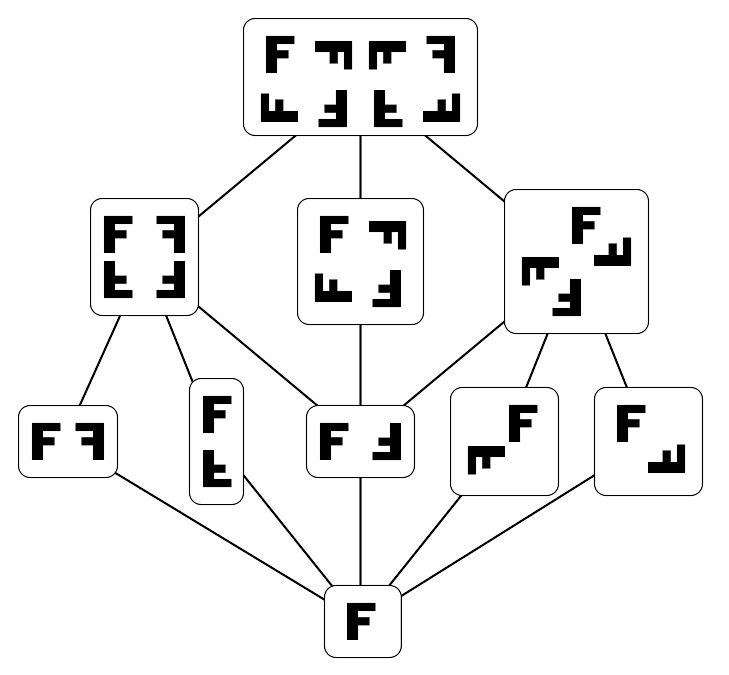
\includegraphics[width=0.25\textwidth]{reticulo-D4}
		\label{fig:reticuloD4dibujo}
		\caption{Retículo de subgrupos de $D_4$ de \cite{d4sub}}
	\end{figure}
	
	\textit{Nos ayudamos de la imágen para sacarlos. La manera de hacerlo sin tener más información que la presentación del grupo es hacerse todos los subgrupos generados por cada elemento y descartar los que son iguales. Luego hacerse todos los subgrupos generados por dos elementos y descartar los que son iguales. Por alguna razón no hace falta probar con los generados por más de dos elementos. Una vez obtenidos estos grupos establecemos las relaciones de inclusión y creamos el diagrama de Hasse.}
\end{ej}

\begin{ej}
	Retículo de subgrupos del grupo de cuaterniones $H$ (figura \ref{fig:reticulocuaterniones})
	
	\begin{figure}[h]
		\centering
		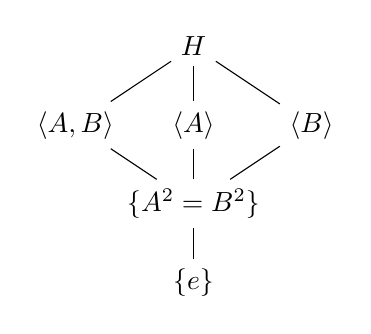
\begin{tikzpicture}
		\node (H) at (0,3) {$H$};
		\node (ab) at (-1.5, 2) {$\langle A, B\rangle$};
		\node (a) at (0,2) {$\langle A \rangle$};
		\node (b) at (1.5,2) {$\langle B \rangle$};
		\node (b2) at (0,1) {$\{A^2 = B^2\}$};
		\node (e) at (0,0) {$\{e\}$};
		
		\draw (e) -- (b2) -- (a) -- (H);
		\draw (b2) -- (ab) -- (H);
		\draw (b2)-- (b) -- (H);
		\end{tikzpicture}
		\caption{Retículo de subgrupos del grupo de cuaterniones $H$.}
		\label{fig:reticulocuaterniones}
	\end{figure}
\end{ej}

El retículo de subgrupos de $D_5$ lo veremos más adelante (para no llenar todo esto de retículos).

\begin{ej}
	
	Sea $G$ abeliano con $|G| = n = rs$, sea $H < G,\ K < G$ con $|H| = r,\ |K| = s$ y $H\cap K = \{e\}$.
	\begin{itemize}
		\item Notemos que como $G$ es abeliano, $H$ y $K$ son subgrupos normales.
		\item Al aplicar el teorema $\ref{thm:cardinalidadproductolibre}$ tenemos que el denominador es $|H\cap K| = 1$ por lo que $|HK| = |H| |K| = rs= n$.
		\item Como $G$ es abeliano:
		\begin{enumerate}
			\item $G = HK$ (porque $HK$ es un subgrupo con el mismo número de elementos que $G$ por el teorema \ref{thm:cardinalidadproductolibre})
			\item La función $f:H\times K \to G,\ (h, k)\mapsto hk$ es un homomorfismo de grupos (nótese que esto no ocurriría si $G$ no fuese abeliano).
		\end{enumerate}
	\end{itemize}
	
	Es más, si se cumple todo lo anterior, $f$ es además un isomorfismo $\implies H\times K \isom G$.
\end{ej}

\begin{ej}
	\label{ej:nohomoentreproducto}
	Consideramos $S_3$, que tiene $|S_3| = 6$ y no es abeliano y los subgrupos $H = \langle (12) \rangle$ y $K = \langle (123) \rangle$ con $|H| = 2$ y $|K| = 3$. Podemos construir la función $f:H\times K \to S_3$ pero no es un homomorfismo de grupos. De hecho, al ser $K \normsub S_3$, el producto $HK$ es un subgrupo y la función $f$ es una biyección, pero aún así no es compatible con la estructura de grupo.
\end{ej}

\begin{ej}
	Consideramos $D_4$ y un grupo $G$ con $a,b \in G$ donde hemos establecido un homomorfismo que definimos con $f(A) = a$ y $f(B) = b$. Ocurre lo siguiente
	\begin{itemize}
		\item El homomorfismo queda totalmente definido ya que todos los elementos de $D_4$ son palabras en $A$ y $B$ y por la estructura de homomorfismo podemos operar tras aplicar la operación a cada letra. Por ejemplo $f(ABA) = aba$.
		\item Es necesario que $o(a) = 2$ y $o(b) = 4$, de lo contrario no se cumpliría la estructura de homomorfismo entre $D_4$ y $G$.
	\end{itemize}
\end{ej}



\begin{ej}
	Veamos un ejemplo (notamos que $(12)^4 = id$)
	\begin{align*}
	f:\Z/4\Z &\to S_3 \\
	\overline{1} &\mapsto (12) \\
	\overline{2} &\mapsto id = (1) \\
	\overline{3} &\mapsto (12) \\
	\overline{4} = \overline{0} &\mapsto id
	\end{align*}
	
	Observamos que $\text{Hom}(\Z/4\Z, S_3) \subset \text{Hom}(\Z, S_3)$ puesto que al tomar $\Z/4\Z$ no podemos tomar cualquier $a$ sino que tenemos que asegurarnos de que $o(a) = o(1)$ (en este caso $o(a) = 2$ pero sigue funcionando porque lo que importa es que $a^{o(1)} = id$).
\end{ej}

Queremos analizar los homomorfismos $f:\ZnZ \to \ZnZ$. Ahora no importa el $\overline{a}$ que elijamos para que $f$ sea homomorfismo porque $\ima f = \langle \overline{a} \rangle$. 

Para que $f$ sea epimorfismo, necesitamos que $\ima f = \langle \overline{a} \rangle = \ZnZ$ es decir que $o(a)$ sea coprimo con $n$.

Concluímos que $\text{Aut}(\ZnZ) \subset \text{Hom}(\ZnZ, \ZnZ)$.

